\documentclass[10pt]{article}

% ---------------------------------------------------------------------------
% Kraken Team -- Quantathon Challenge #1 -- Technical Report
% Compile with pdfLaTeX (e.g. Overleaf). No external image files required:
% every flow chart is drawn natively in TikZ, redrawn from docs/diagrams/*.mmd.
% ---------------------------------------------------------------------------

\usepackage[a4paper,margin=2cm]{geometry}
\usepackage[T1]{fontenc}
\usepackage[utf8]{inputenc}
\usepackage{lmodern}
\usepackage{amsmath,amssymb}
\usepackage{booktabs}
\usepackage{graphicx}
\usepackage{xcolor}
\usepackage{caption}
\usepackage{subcaption}
\usepackage[hidelinks]{hyperref}
\usepackage{enumitem}
\usepackage{tikz}
\usetikzlibrary{shapes.geometric,arrows.meta,positioning,fit,backgrounds,calc}
\usepackage{titlesec}

% Resolve figure filenames from both image folders (paths relative to this .tex).
\graphicspath{{../figures/}{../experiments/figures/}}

\setlist{nosep,leftmargin=1.4em}
\titlespacing*{\section}{0pt}{1.0ex plus .2ex}{0.6ex}
\titlespacing*{\subsection}{0pt}{0.8ex plus .2ex}{0.4ex}
\captionsetup{font=small,labelfont=bf,skip=3pt}

% ---- shared TikZ styles for the flow charts -------------------------------
\definecolor{cData}{HTML}{DCE6F5}
\definecolor{cProc}{HTML}{E7F2DC}
\definecolor{cQuant}{HTML}{F5E1DC}
\definecolor{cDec}{HTML}{FBF0D0}
\tikzset{
  node distance=6mm and 10mm,
  data/.style   ={rectangle, rounded corners=2pt, draw=black!55, fill=cData,
                  align=center, font=\scriptsize, inner sep=3pt, minimum height=7mm},
  proc/.style   ={rectangle, draw=black!55, fill=cProc, align=center,
                  font=\scriptsize, inner sep=3pt, minimum height=7mm},
  quant/.style  ={rectangle, draw=black!55, fill=cQuant, align=center,
                  font=\scriptsize, inner sep=3pt, minimum height=7mm},
  dec/.style    ={diamond, aspect=2, draw=black!55, fill=cDec, align=center,
                  font=\scriptsize, inner sep=1pt},
  fl/.style     ={-{Stealth[length=2mm]}, draw=black!65},
  lbl/.style    ={font=\scriptsize\itshape, fill=white, inner sep=1pt},
}

\title{\vspace{-1.2cm}\textbf{Quantum Fault-Zone Partitioning of the Costa Rican
Power Grid}\\[2pt]\large A Max-Cut / QAOA Study --- Quantathon Challenge \#1}
\author{Kraken Team --- Gabriel Alba Romero, Juan C.\ Lara}
\date{\today}

\begin{document}
\maketitle
\vspace{-0.7cm}

% ===========================================================================
\section{Problem framing}
% ===========================================================================

\paragraph{Physical problem.} A transmission grid must be split into
self-sufficient \emph{fault zones}: when a fault occurs, protection relays open
a small set of tie-lines so the faulted region can be isolated \emph{without}
severing the lines that carry the most power or that hold the grid together.
A good split therefore (i)~cuts as little critical transmission capacity as
possible and (ii)~leaves generation on \emph{both} sides so neither zone goes
dark. We model this as a \textbf{graph-partitioning / Max-Cut} problem on the
Costa Rican national grid and solve it both classically and with QAOA.

\paragraph{Graph model} We snapshot two open ICE ArcGIS layers ---
\emph{Subestaciones} (substations) and \emph{L\'ineas de Transmisi\'on}
(transmission lines) --- into a static, reproducible dataset and build a
weighted undirected graph $G=(V,E)$. Substations become nodes; each line's
\texttt{Circuito} field (``SubA--SubB'') yields an edge. Parallel lines are
collapsed (weights summed, highest voltage kept), and endpoints with no matching
substation (international ties, SIEPAC, industrial loads) are marked as
\emph{border} nodes. The national graph has $75$ nodes and $97$ edges. Because
exact solutions and today's emulators are limited to a modest qubit count, we
deterministically extract a connected sub-region --- \textbf{Guanacaste North},
$n=9$ substations, $9$ lines, $1$ independent cycle, $7$ of which host
generation (max plant $306.2$\,MW).

\paragraph{Edge weights} Every edge weight measures \emph{how
costly it is to cut that line}. Weight schemes are a registry of pure functions
\texttt{fn(voltage, length, gens\_u, gens\_v)}; the project default,
\texttt{generation\_inverted}, is generator-aware and sign-inverted so that the
\emph{most critical} lines carry the \emph{largest positive} weight
($w_{\max}=16.106$ for this sub-grid). This lets a \emph{minimize-cut} objective
directly express ``protect the critical lines.''

\paragraph{Pipeline.} The project is a linear, reproducible flow from raw ICE
data to a quantum-ready cost Hamiltonian and a classical/quantum comparison
(Fig.~\ref{fig:pipeline}). Task~A produces the weighted sub-graph, Task~B the
QUBO / Ising / cost Hamiltonian, Task~C the QAOA solver; classical baselines
score the \emph{same} operator for a fair comparison.

\begin{figure}[t]
\centering
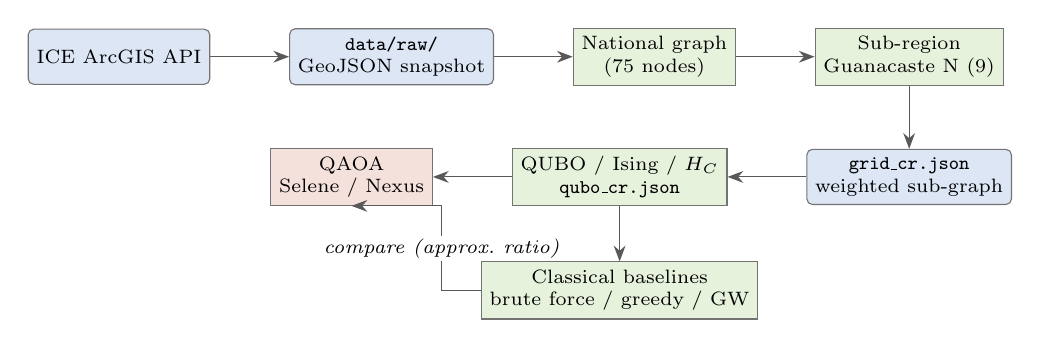
\begin{tikzpicture}
  \node[data]  (ice)  {ICE ArcGIS API};
  \node[data,right=of ice] (raw) {\texttt{data/raw/}\\GeoJSON snapshot};
  \node[proc,right=of raw] (nat) {National graph\\(75 nodes)};
  \node[proc,right=of nat] (sub) {Sub-region\\Guanacaste N (9)};
  \node[data,below=8mm of sub] (json){\texttt{grid\_cr.json}\\weighted sub-graph};
  \node[proc,left=of json] (qubo){QUBO / Ising / $H_C$\\\texttt{qubo\_cr.json}};
  \node[quant,left=of qubo] (qaoa){QAOA\\Selene / Nexus};
  \node[proc,below=7mm of qubo] (base){Classical baselines\\brute force / greedy / GW};

  \draw[fl] (ice)--(raw); \draw[fl] (raw)--(nat); \draw[fl] (nat)--(sub);
  \draw[fl] (sub)--(json); \draw[fl] (json)--(qubo); \draw[fl] (qubo)--(qaoa);
  \draw[fl] (qubo)--(base);
  \draw[fl] (base.west) -- ++(-0.5,0) |- (qaoa.south)
        node[lbl,pos=0.25]{compare (approx.\ ratio)};
\end{tikzpicture}
\caption{End-to-end pipeline. Blue = data artifacts, green = classical
processing, red = quantum. Only the static snapshot is ever read downstream, so
every run is reproducible.}
\label{fig:pipeline}
\end{figure}

\begin{figure}[t]
\centering
\begin{subfigure}[b]{0.46\textwidth}
\centering

\includegraphics[height=5.2cm]{national_grid.png}
\caption{National grid; the Guanacaste-North sub-grid highlighted in green.}
\label{fig:grid-national}
\end{subfigure}\hfill
\begin{subfigure}[b]{0.50\textwidth}
\centering

\includegraphics[height=5.2cm]{guanacaste_north_subgrid.png}
\caption{The extracted $9$-node sub-region ($9$ lines, $1$ cycle) solved by
Max-Cut / QAOA.}
\label{fig:grid-sub}
\end{subfigure}
\caption{From the full ICE transmission grid (Task~A) to the deterministic
connected sub-region used throughout the study.}
\label{fig:grids}
\end{figure}

% ===========================================================================
\section{Classical formulation and baselines}
% ===========================================================================

\subsection{QUBO / Ising / cost Hamiltonian}
Each node gets a binary variable $x_i\in\{0,1\}$ labelling its fault zone. The
weight of the cut is
\[
\mathrm{Cut}(x)=\sum_{(i,j)\in E} w_{ij}\,(x_i+x_j-2x_ix_j),
\]
where the bracket is $1$ exactly when the edge is cut. We \emph{minimize}
$\mathrm{Cut}(x)$ (not maximize): with the inverted-generation weights, cutting a
critical line is expensive, so the boundary settles on the cheapest tie-lines.
Two \textbf{quadratic} (ancilla-free) penalties, registered like the weight
schemes, encode the operational constraints:
\begin{itemize}
  \item \emph{Generator spread} $P_{\text{gen}}\sum_{\text{gen pairs}}(1-\text{cut}_{ij})$
        --- keeps generation on both sides; symmetric, so it excludes both
        trivial all-same partitions. $P_{\text{gen}}=0.5\,w_{\max}$ per pair.
  \item \emph{Balance} $\lambda(\sum_i x_i-n/2)^2$ --- discourages lopsided
        cuts. $\lambda=0.15\,w_{\max}$.
\end{itemize}
The accumulated QUBO $\mathrm{cost}(x)=\sum_i Q_{ii}x_i+\sum_{i<j}Q_{ij}x_ix_j+
\text{offset}$ is mapped to spins via $x_i=(1-z_i)/2$, giving the diagonal
\textbf{cost Hamiltonian}
\[
H_C=\text{offset}\cdot I+\sum_i h_i Z_i+\sum_{i<j}J_{ij}Z_iZ_j .
\]
Because every term is at most two-local $Z$, $H_C$ is diagonal in the
computational basis: its ground state \emph{is} the optimal fault-zone
partition, and \texttt{QUBO.energy}, \texttt{CostHamiltonian.energy}, and the
brute-force enumerator agree bit-for-bit. This single operator is what
\emph{every} solver --- classical and quantum --- is scored on
(Fig.~\ref{fig:formulation}).

\begin{figure}[t]
\centering
\begin{subfigure}[t]{0.52\textwidth}
\centering
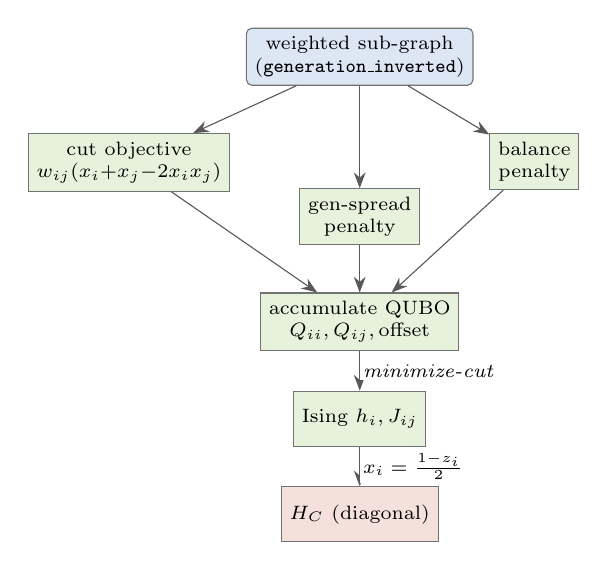
\begin{tikzpicture}[node distance=4.5mm and 7mm]
  \node[data] (g) {weighted sub-graph\\(\texttt{generation\_inverted})};
  \node[proc,below left=6mm and 2mm of g] (obj){cut objective\\$w_{ij}(x_i{+}x_j{-}2x_ix_j)$};
  \node[proc,below=13mm of g] (gen){gen-spread\\penalty};
  \node[proc,below right=6mm and 2mm of g] (bal){balance\\penalty};
  \node[proc,below=6mm of gen] (acc){accumulate QUBO\\$Q_{ii},Q_{ij},\text{offset}$};
  \node[proc,below=5mm of acc] (is){Ising $h_i,J_{ij}$};
  \node[quant,below=5mm of is] (hc){$H_C$ (diagonal)};
  \draw[fl](g)--(obj);\draw[fl](g)--(gen);\draw[fl](g)--(bal);
  \draw[fl](obj)--(acc);\draw[fl](gen)--(acc);\draw[fl](bal)--(acc);
  \draw[fl](acc)--(is) node[lbl,midway,right]{minimize-cut};
  \draw[fl](is)--(hc) node[lbl,midway,right]{$x_i=\tfrac{1-z_i}{2}$};
\end{tikzpicture}
\caption{QUBO formulation (Task~B).}
\label{fig:formulation-a}
\end{subfigure}\hfill
\begin{subfigure}[t]{0.45\textwidth}
\centering
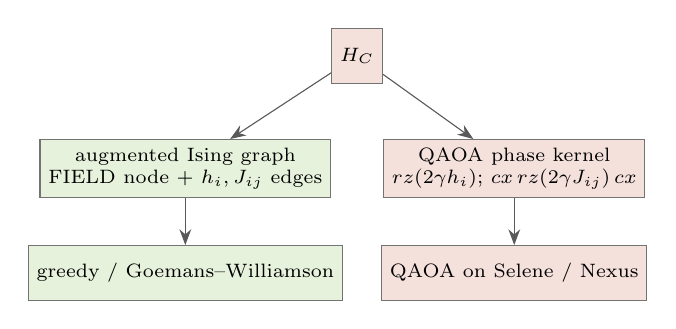
\begin{tikzpicture}[node distance=5mm and 6mm]
  \node[quant] (hc) {$H_C$};
  \node[proc,below left=7mm and 0mm of hc] (aug){augmented Ising graph\\FIELD node $+$ $h_i,J_{ij}$ edges};
  \node[quant,below right=7mm and 0mm of hc] (ker){QAOA phase kernel\\$rz(2\gamma h_i)$; $cx\,rz(2\gamma J_{ij})\,cx$};
  \node[proc,below=6mm of aug] (cls){greedy / Goemans--Williamson};
  \node[quant,below=6mm of ker] (qa){QAOA on Selene / Nexus};
  \draw[fl](hc)--(aug);\draw[fl](hc)--(ker);
  \draw[fl](aug)--(cls);\draw[fl](ker)--(qa);
\end{tikzpicture}
\caption{One $H_C$, two consumers: the augmented Max-Cut graph feeds the
classical baselines, the phase kernel feeds QAOA.}
\label{fig:formulation-b}
\end{subfigure}
\caption{From weighted graph to a single diagonal cost Hamiltonian scored by
both families of solvers.}
\label{fig:formulation}
\end{figure}

\subsection{Classical baselines}
All classical solvers optimize the \emph{same} objective by running on
\texttt{augmented\_ising\_graph($H_C$)}, a weighted Max-Cut graph (a FIELD node
carrying the fields $h_i$ plus $J_{ij}$ edges) whose maximum cut equals
minimizing $\langle H_C\rangle$; partitions map back with
\texttt{bits\_from\_partition}.
\begin{itemize}
  \item \textbf{Brute force (exact reference).} A single vectorized enumerator
        (\texttt{enumerate\_cut\_spectrum}) sweeps all $2^{n}$ assignments in
        NumPy chunks, pinning one node (global-flip symmetry) so only $2^{n-1}$
        are visited and peak memory stays proportional to the chunk. It yields
        the exact spectrum bounds $(e_{\min},e_{\max})$ that anchor every score;
        a $300$\,s timeout falls back to a Goemans--Williamson proxy beyond
        $\sim\!26$ qubits.
  \item \textbf{Greedy (heuristic lower bar).} Visits nodes in a seeded random
        order, placing each on the side that maximizes immediate cut gain.
        As a sampler it runs \texttt{n\_shots} independent seeded restarts ---
        the same sample budget as QAOA shots.
  \item \textbf{Goemans--Williamson (strongest baseline).} Solves the SDP
        relaxation $\max\sum W_{ij}(1-X_{ij})/2$ s.t.\ $\mathrm{diag}(X)=1,\,
        X\succeq0$ (cvxpy + SCS) \emph{once}, then performs \texttt{n\_shots}
        random-hyperplane roundings, carrying the classic $0.878$ guarantee for
        non-negative weights.
\end{itemize}
Every solver produces bit assignments scored by the \textbf{offset-robust
approximation ratio}
$r=(e_{\max}-E)/(e_{\max}-e_{\min})$, so $r=1$ is the classical optimum and
different signs/offsets are comparable (Fig.~\ref{fig:optimizers}).

\begin{figure}[t]
\centering
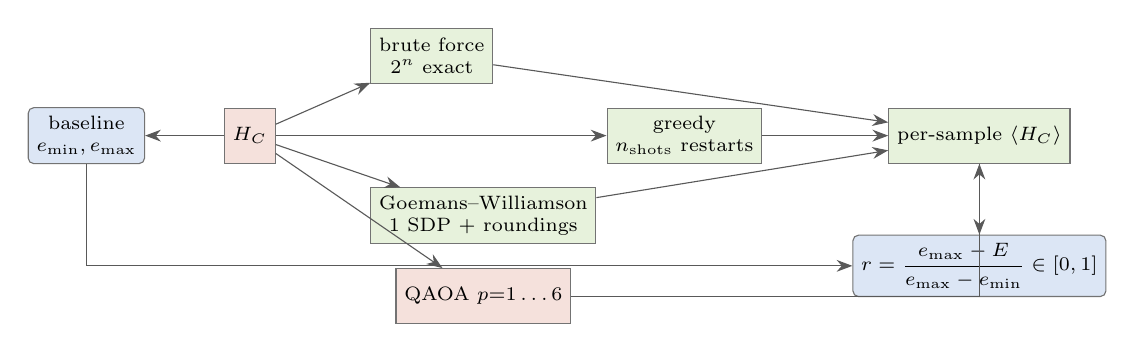
\begin{tikzpicture}[node distance=4mm and 8mm]
  \node[quant] (hc) {$H_C$};
  \node[proc,above right=3mm and 12mm of hc] (bf){brute force\\$2^n$ exact};
  \node[proc,right=42mm of hc] (gr){greedy\\$n_{\text{shots}}$ restarts};
  \node[proc,below right=3mm and 12mm of hc] (gw){Goemans--Williamson\\1 SDP $+$ roundings};
  \node[quant,below=3mm of gw] (qa){QAOA $p{=}1\ldots6$};
  \node[data,left=10mm of hc] (base){baseline\\$e_{\min},e_{\max}$};
  \node[proc,right=16mm of gr] (en){per-sample $\langle H_C\rangle$};
  \node[data,below=9mm of en] (ar){$r=\dfrac{e_{\max}-E}{e_{\max}-e_{\min}}\in[0,1]$};
  \draw[fl](hc)--(bf);\draw[fl](hc)--(gr);\draw[fl](hc)--(gw);\draw[fl](hc)--(qa);
  \draw[fl](hc)--(base);
  \draw[fl](bf)--(en);\draw[fl](gr)--(en);\draw[fl](gw)--(en);
  \draw[fl](qa.east)-|(en);
  \draw[fl](en)--(ar);\draw[fl](base)|-(ar);
\end{tikzpicture}
\caption{Every optimizer scores the same $H_C$; the brute-force spectrum bounds
turn each energy into a comparable approximation ratio.}
\label{fig:optimizers}
\end{figure}

\begin{figure}[t]
\centering
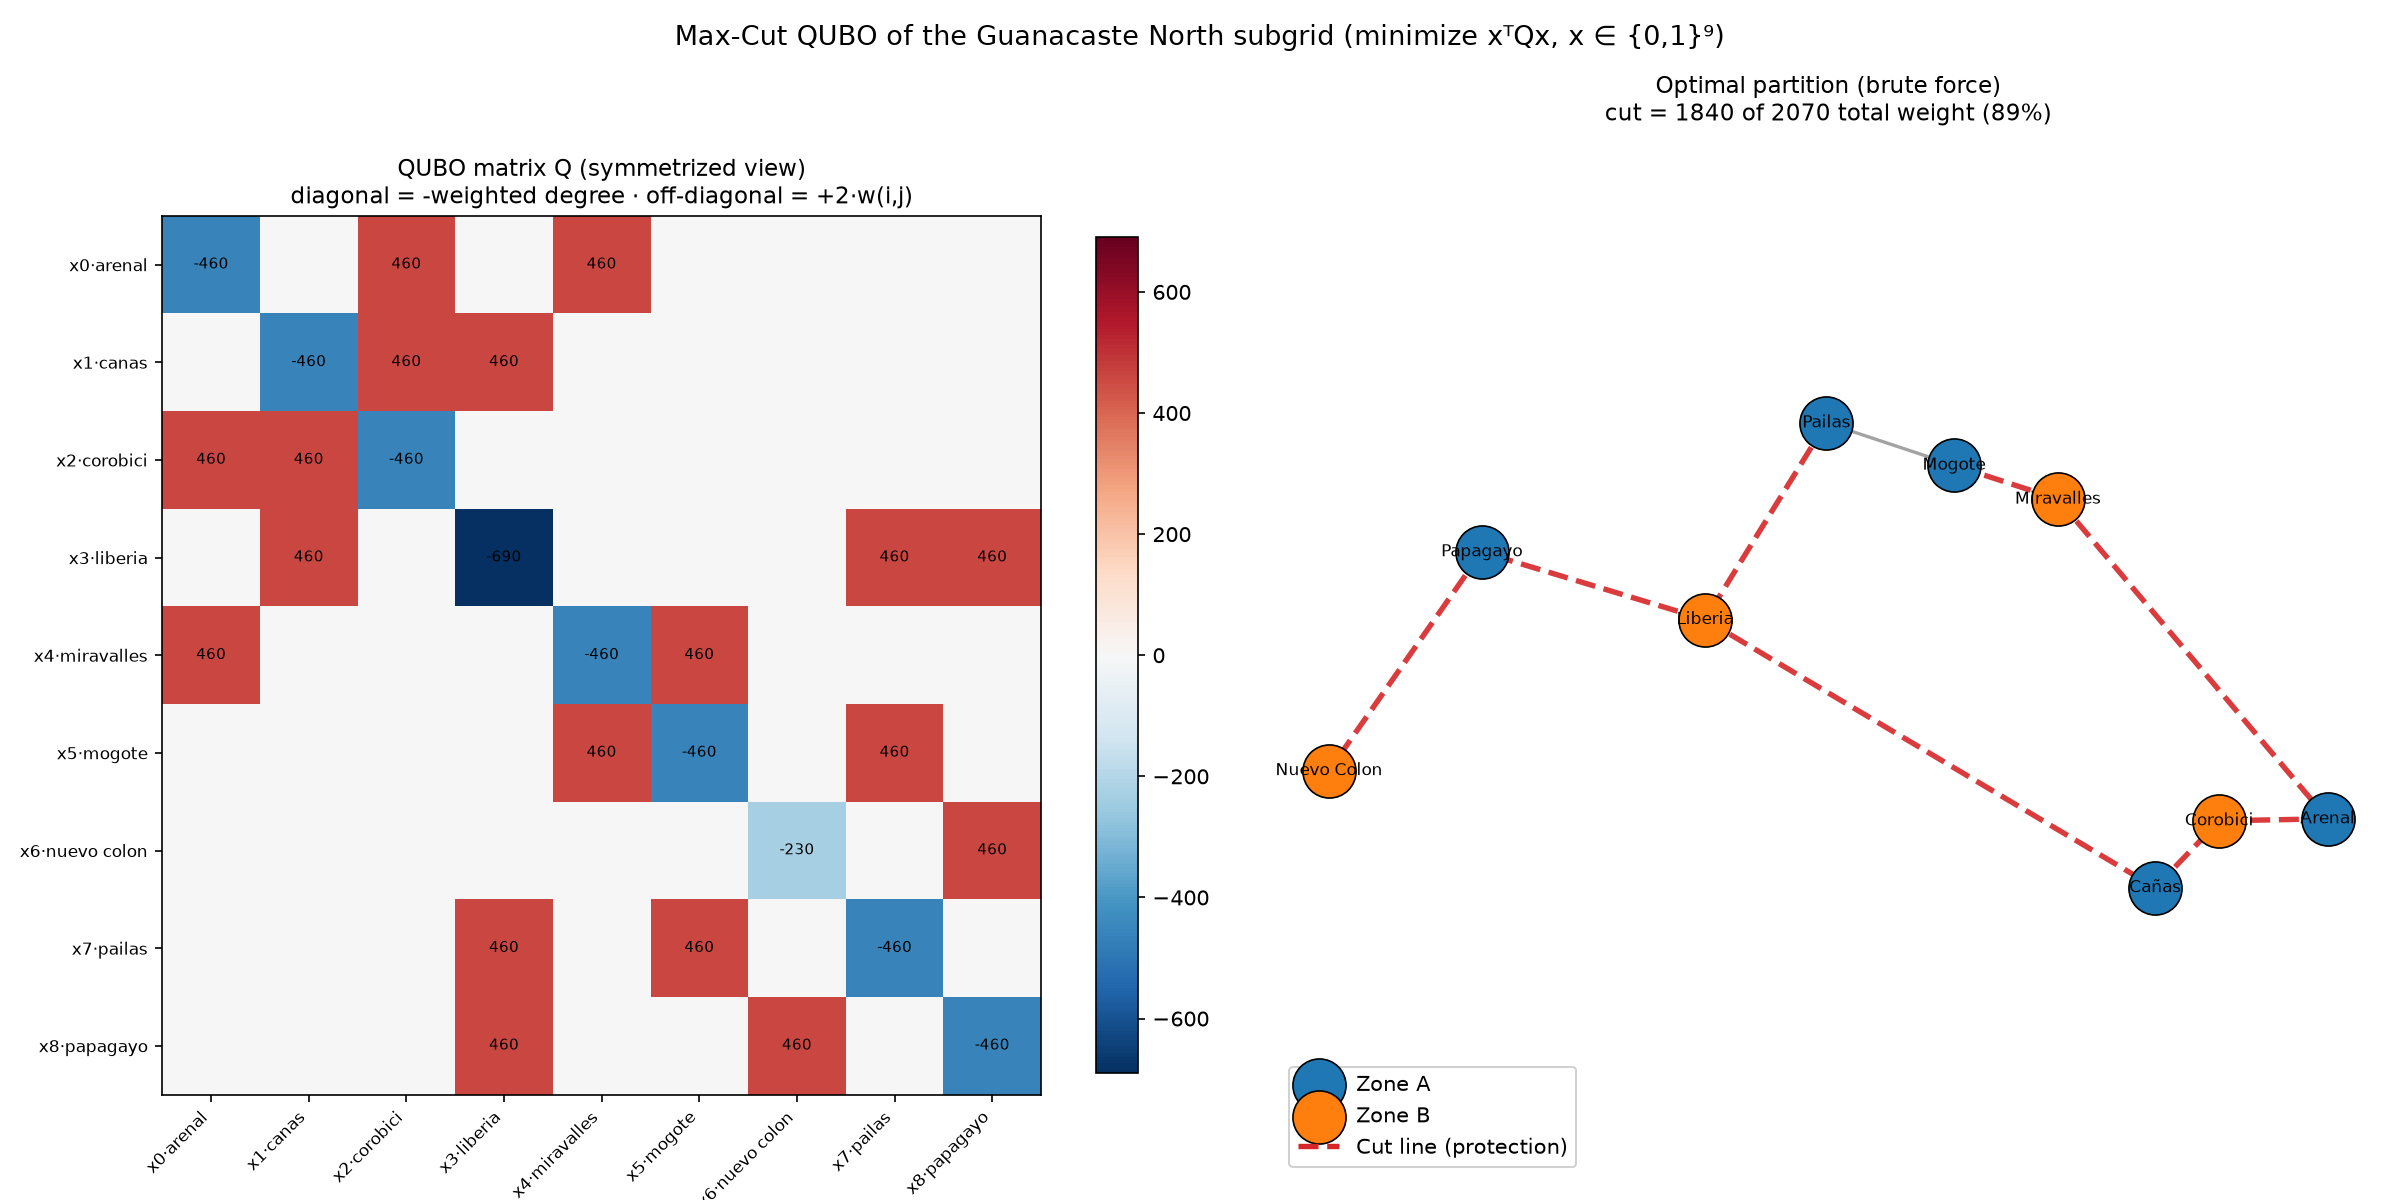
\includegraphics[width=0.95\textwidth]{qubo_maxcut.png}
\caption{The QUBO for the Guanacaste-North sub-grid: the symmetrized $Q$ matrix
(left) and the exact brute-force optimal fault-zone partition (right), with the
protected zone boundary drawn as dashed cut lines.}
\label{fig:qubo-maxcut}
\end{figure}

% ===========================================================================
\section{Quantum implementation}
% ===========================================================================

We solve the fault-zone problem with the \textbf{Quantum Approximate
Optimization Algorithm (QAOA)}, written in \textbf{Guppy~0.21} and executed on
the \textbf{Selene} emulator (locally) or the \textbf{Quantinuum Nexus} hosted
emulator (Helios). The number of qubits ($9$), the operator $H_C$, and even the
\emph{minimize} direction are fixed by the QUBO --- not free choices.

\paragraph{Weighted phase/mixer kernel.} Because $H_C$ is weighted and carries
single-$Z$ fields, we cannot reuse the unweighted Max-Cut example kernel.
Following the diagonal-$H_C$ mapping, one QAOA layer applies

\smallskip
\begin{tabular}{@{}ll@{}}
\toprule
Term & Circuit fragment\\
\midrule
$h_i Z_i$ (field)      & $rz(2\gamma h_i,\,i)$\\
$J_{ij}Z_iZ_j$ (coupling) & $cx(i,j);\ rz(2\gamma J_{ij},\,j);\ cx(i,j)$\\
mixer                  & $rx(2\beta,\,i)$ per qubit\\
$\text{offset}\cdot I$ & global phase --- ignored\\
\bottomrule
\end{tabular}
\smallskip

\noindent Coefficients are baked in as \texttt{comptime} constants. A Guppy~0.21
subtlety: \texttt{angle(x)} means $x$ \emph{half-turns} ($x\pi$ rad), so each
$2h_i$ (and the mixer's $2$) is folded with a $1/\pi$ factor at compile time to
keep the radian convention while $\gamma,\beta$ stay plain multipliers. Empty
term lists are padded with a zero-coefficient placeholder ($rz(0)$ is identity)
because Guppy cannot type-infer an empty \texttt{comptime} list.

\paragraph{Variational loop.} Energy is the true expectation $\langle
H_C\rangle$ from \texttt{CostHamiltonian.energy} weighted by shot
probabilities. \textbf{SciPy COBYLA} minimizes it over the flattened
$[\gamma(p),\beta(p)]$ parameters; a fixed seed makes every emulator evaluation
deterministic (Fig.~\ref{fig:qaoa}). The kernel is backend-agnostic: it compiles
to HUGR and runs on local Selene (\texttt{main.emulator(...).run()}) or Nexus
(\texttt{upload}$\to$\texttt{start\_execute\_job}$\to$\texttt{wait\_for}), which
return the \emph{same} \texttt{QsysResult} type, so decoding is identical. For
$n\le12$ the exact ground state (\texttt{brute\_force\_ground\_state}) and
spectrum bounds provide the reference for the approximation ratio.

\begin{figure}[t]
\centering
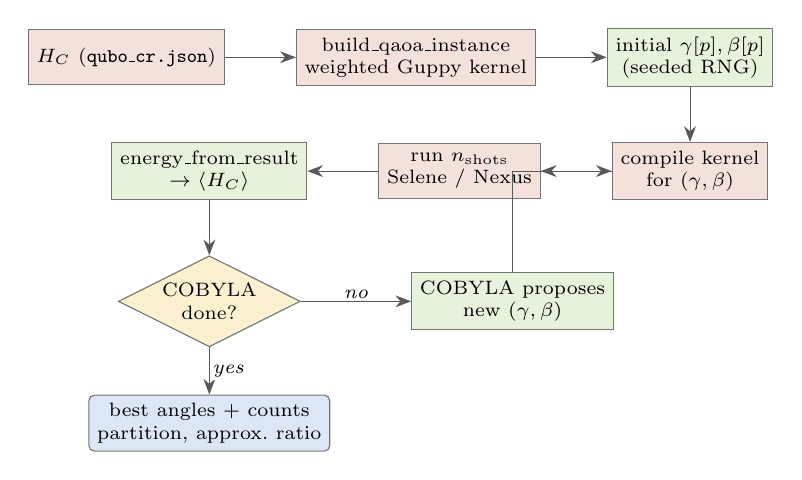
\begin{tikzpicture}[node distance=5mm and 9mm]
  \node[quant] (hc) {$H_C$ (\texttt{qubo\_cr.json})};
  \node[quant,right=of hc] (bi) {build\_qaoa\_instance\\weighted Guppy kernel};
  \node[proc,right=of bi] (init) {initial $\gamma[p],\beta[p]$\\(seeded RNG)};
  \node[quant,below=7mm of init] (comp) {compile kernel\\for $(\gamma,\beta)$};
  \node[quant,left=of comp] (run) {run $n_{\text{shots}}$\\Selene / Nexus};
  \node[proc,left=of run] (en) {energy\_from\_result\\$\to\langle H_C\rangle$};
  \node[dec,below=7mm of en] (conv) {COBYLA\\done?};
  \node[proc,right=14mm of conv] (new) {COBYLA proposes\\new $(\gamma,\beta)$};
  \node[data,below=6mm of conv] (out) {best angles $+$ counts\\partition, approx.\ ratio};
  \draw[fl](hc)--(bi);\draw[fl](bi)--(init);\draw[fl](init)--(comp);
  \draw[fl](comp)--(run);\draw[fl](run)--(en);\draw[fl](en)--(conv);
  \draw[fl](conv)-- node[lbl,above]{no} (new);
  \draw[fl](new)|-(comp);
  \draw[fl](conv)-- node[lbl,right]{yes} (out);
\end{tikzpicture}
\caption{QAOA variational loop. COBYLA drives the $(\gamma,\beta)$ search;
each evaluation compiles the weighted kernel, samples the emulator, and decodes
$\langle H_C\rangle$.}
\label{fig:qaoa}
\end{figure}

\begin{figure}[t]
\centering
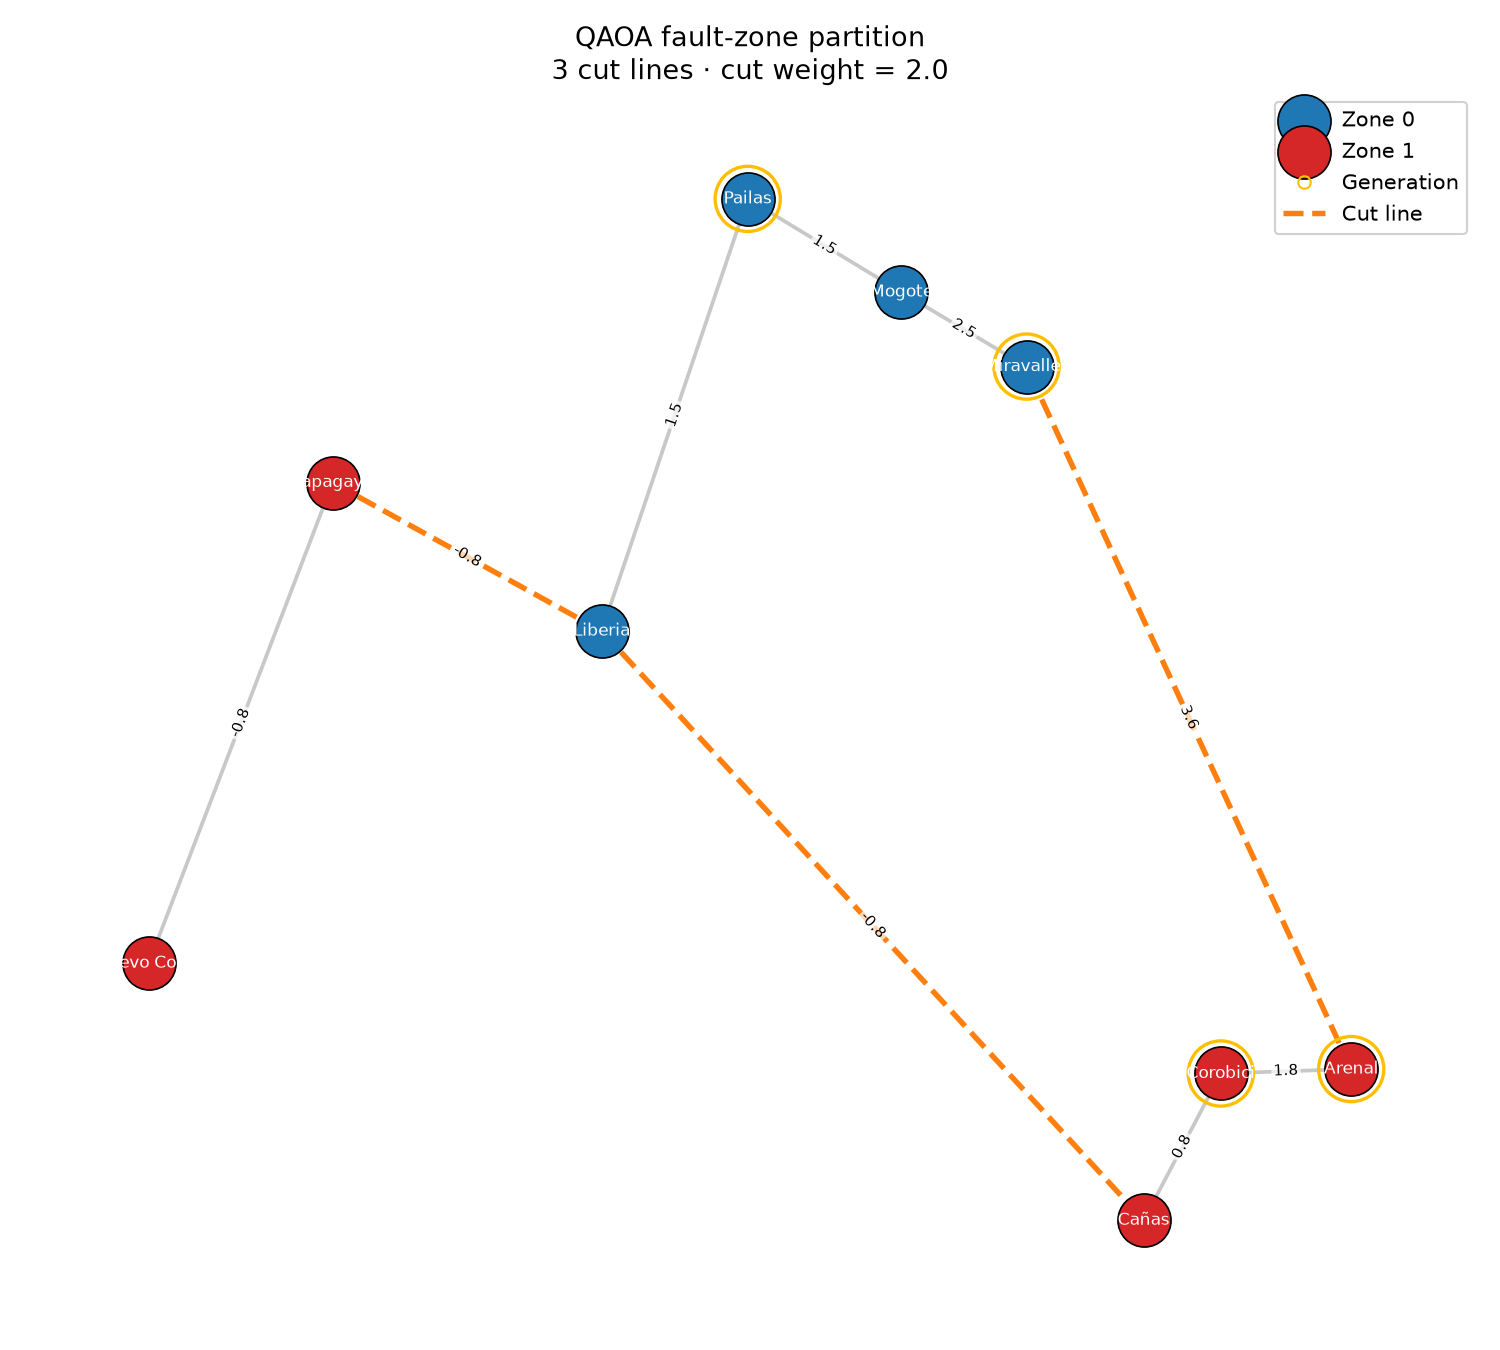
\includegraphics[width=0.62\textwidth]{qaoa_partition.png}
\caption{Fault-zone partition recovered by QAOA on the sub-grid: nodes coloured
by zone, generation-bearing substations ringed, and the cut (protected boundary)
lines dashed.}
\label{fig:qaoa-partition}
\end{figure}

% ===========================================================================
\section{Results}
% ===========================================================================

% ---------------------------------------------------------------------------
% RESULTS TABLE -- pre-populated from experiments/results/
%   evaluation_20260724_072452.json (Guanacaste North, n=9, 3 replicate runs,
%   1000 shots, COBYLA maxiter=40). Update numbers if you re-run the benchmark.
% ---------------------------------------------------------------------------
\begin{table}[h]
\centering
\small
\caption{Comparison on the Guanacaste-North instance ($n=9$, $e_{\min}=4.96$,
$e_{\max}=21.54$). Mean $\pm$ std over $3$ replicate runs, $1000$ shots each.
$r$ = approximation ratio ($1$ = classical optimum). Best-of-run $r$ shown
separately from the mean-over-samples $r$.}
\label{tab:results}
\begin{tabular}{@{}lccccc@{}}
\toprule
Optimizer & Best energy & Mean $r$ & Best $r$ & MSE vs.\ opt. & Time (s)\\
\midrule
Goemans--Williamson & $4.96\pm0.00$ & $0.962\pm0.001$ & $1.000\pm0.000$ & $0.64\pm0.02$ & $1.9\pm1.3$\\
Greedy              & $4.96\pm0.00$ & $0.939\pm0.001$ & $1.000\pm0.000$ & $1.64\pm0.03$ & $2.0\pm1.3$\\
QAOA $p=1$          & $5.15\pm0.26$ & $0.676\pm0.004$ & $0.989\pm0.016$ & $39.1\pm0.7$  & $170\pm13$\\
QAOA $p=3$          & $5.15\pm0.26$ & $0.733\pm0.075$ & $0.989\pm0.016$ & $29.4\pm12.3$ & $290\pm4$\\
\bottomrule
\end{tabular}
\end{table}

\paragraph{Reading the table.} The exact optimum ($e_{\min}=4.96$) is reached
by both classical baselines and, in its best shot, by QAOA (best
$r=0.989$--$1.0$). The \emph{mean}-over-samples ratio separates the methods:
Goemans--Williamson concentrates near the optimum ($0.962$), greedy trails
slightly ($0.939$), and shallow QAOA has a broader shot distribution
($0.676$ at $p=1$, rising to $0.733$ at $p=3$) --- deeper circuits sharpen the
distribution toward the optimum, at higher runtime. Error bars come from the
$3$ replicate runs (independent seeds); the classical baselines are essentially
deterministic on this instance while QAOA shows the expected run-to-run variance.

% ---------------------------------------------------------------------------
% PLACEHOLDER -- figures. Drop the generated PNGs / plots here.
%   Suggested sources:
%     figures/qaoa_partition.png      -- QAOA fault-zone partition of the sub-grid
%     figures/qubo_maxcut.png         -- classical Max-Cut partition
%     figures/guanacaste_north_*.png  -- the sub-region and its plants
%   Plus, from notebooks/evaluation.ipynb:
%     energy-distribution histograms, approximation-ratio box plots (error bars),
%     and approximation-ratio convergence curves.
% ---------------------------------------------------------------------------
\begin{figure}[h]
\centering
\begin{subfigure}[t]{\textwidth}
\centering
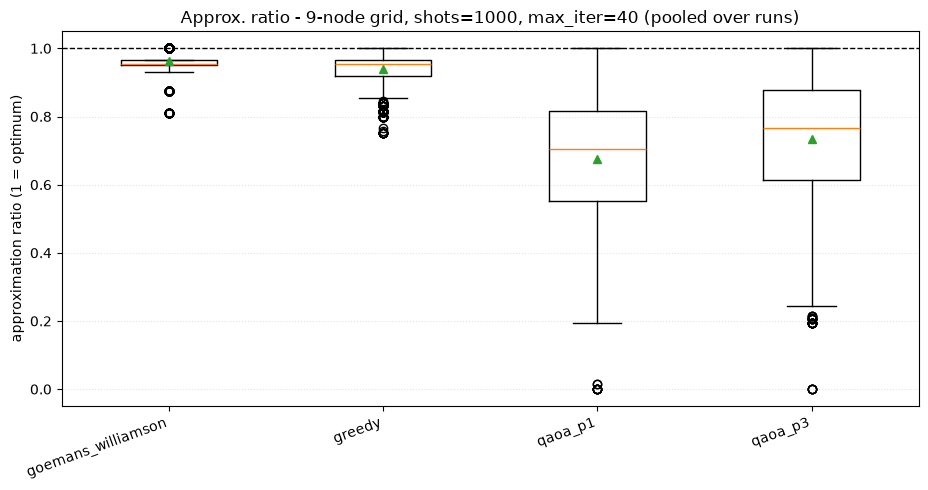
\includegraphics[width=0.82\textwidth]{box_plot.png}
\caption{Approximation-ratio distribution per optimizer (box = interquartile
range, whiskers, green triangle = mean); $1.0$ is the classical optimum.}
\label{fig:res-box}
\end{subfigure}

\medskip
\begin{subfigure}[t]{0.49\textwidth}
\centering
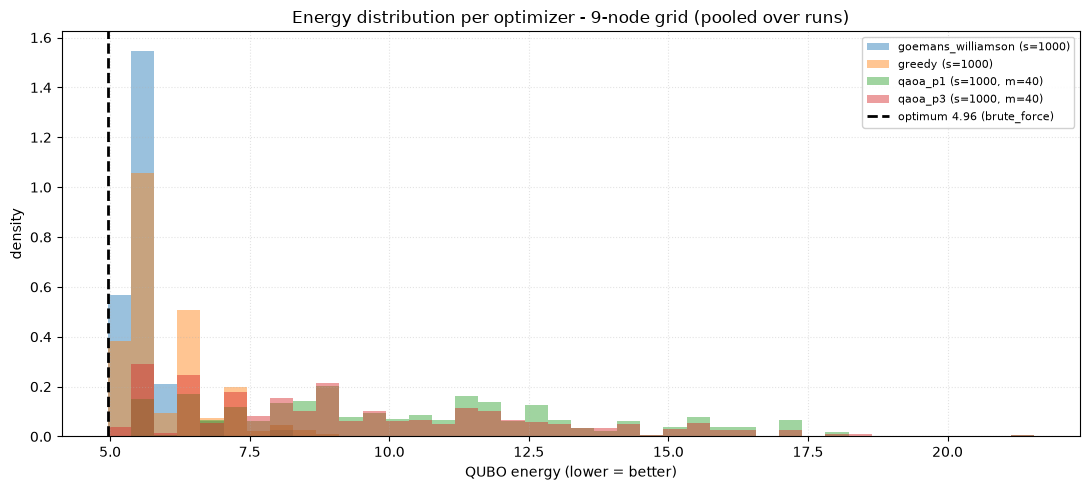
\includegraphics[width=\textwidth]{distribution.png}
\caption{Pooled per-shot energy distributions; dashed line = brute-force
optimum $4.96$.}
\label{fig:res-dist}
\end{subfigure}\hfill
\begin{subfigure}[t]{0.49\textwidth}
\centering
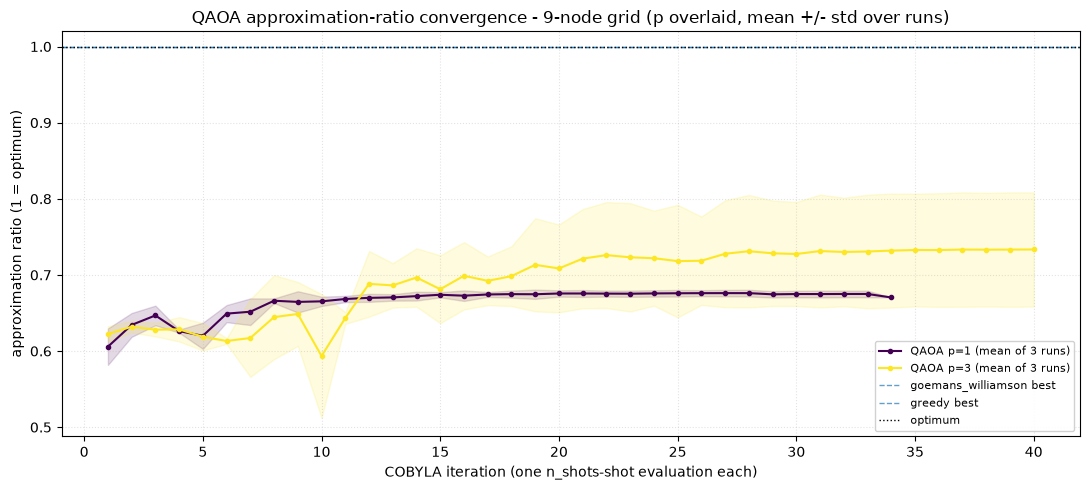
\includegraphics[width=\textwidth]{convergence.png}
\caption{QAOA approximation-ratio convergence vs.\ COBYLA iteration, mean $\pm$
std over the $3$ replicate runs.}
\label{fig:res-conv}
\end{subfigure}
\caption{Results on the Guanacaste-North instance ($n=9$, $1000$ shots, $3$
replicate runs). Error bars/spreads come from the replicate runs and the shot
distributions.}
\label{fig:results}
\end{figure}

\paragraph{Analysis.}
% ---------------------------------------------------------------------------
% PLACEHOLDER -- results analysis prose (to be written).
% Discuss: approximation-ratio trend vs p, effect of shots, convergence
% behaviour, classical vs quantum gap, and what the chosen partition means
% physically (which tie-lines are cut, generation balance across zones).
% ---------------------------------------------------------------------------
\emph{[PLACEHOLDER --- add your analysis of the figures above: the
approximation-ratio trend with circuit depth $p$, convergence behaviour, the
classical/quantum gap, and the physical interpretation of the chosen
partition.]}

% ===========================================================================
\section{Honest limitations}
% ===========================================================================
% ---------------------------------------------------------------------------
% PLACEHOLDER -- to be completed by the author.
% Candidate points to cover (edit / expand as you see fit):
%   * Problem scale: 9-qubit sub-region, not the full 75-node national grid;
%     brute force capped at ~26 qubits.
%   * Emulation, not hardware: Selene / Nexus emulator results; no real device
%     noise, gate errors, or connectivity constraints.
%   * Shallow QAOA is heuristic: no optimality guarantee; mean approx. ratio
%     below the classical baselines at small p.
%   * Model fidelity: weights are a proxy for line criticality; snapshot data,
%     name-matching heuristics, dropped border nodes.
%   * Optimizer: COBYLA local minima, limited maxiter, fixed seed.
% ---------------------------------------------------------------------------
During the execution of the hackathon there were a few limitations that were found. In the first place, from our baseline case of 9 nodes to the max possible 26 qubits QAOA scales in a very steep fashion, making it unfeasible to be able to run as many evaluations as we wanted. Additionally, the speed of the emulators was a huge bottleneck when trying to run optimizations since a single cycle was needed for every optimization iteration, which meant we had to end up defaulting to using Selene local emulation instead of Nexus' backends. There is a small caveat here, where our web-app does run in the Nexus backend. Likewise, we also faced a big limitation in terms of time. Since none of the team members had any physics or quantum computing background, most of the first day had to be spent in gaining a better understanding of the QAOA optimizer and what the problem was at it's core, which in the end meant less time for running evaluations.

\end{document}
